\documentclass{ctexart}
\usepackage[T1]{fontenc}
\usepackage[a4paper,top=1.5cm,bottom=1.5cm,left=2cm,right=2cm,marginparwidth=1.75cm]{geometry}
\usepackage{mathtools}
\usepackage{booktabs}
\usepackage{caption}
\usepackage{outlines}
\usepackage{graphicx}
\usepackage[colorlinks=false, allcolors=blue]{hyperref}
\renewcommand{\tableautorefname}{表}
\DeclarePairedDelimiter{\set}{\{}{\}}
\DeclarePairedDelimiter{\paren}{(}{)}
\graphicspath{ {./images/} }

\title{微机接口第二次作业}
\author{卢雨轩 19071125}
% \date{\today}
\ctexset{
    section = {
        titleformat = \raggedright,
        name = {,},
        number = \chinese{section}、
    },
    paragraph = {
        runin = false
    },
    today = small,
    figurename = 图,
    contentsname = 目录,
    tablename = 表,
}

\begin{document}

\maketitle

某一个微机系统中,有4块I/O接口芯片,每个芯片占有8个端口地址,若起始地址为100H,8块芯片的地址连续分布,用可采用多片74LS138和74LS04设计译码电路,试画出端口译码电路,并说明每块芯片的端口地址范围。

\noindent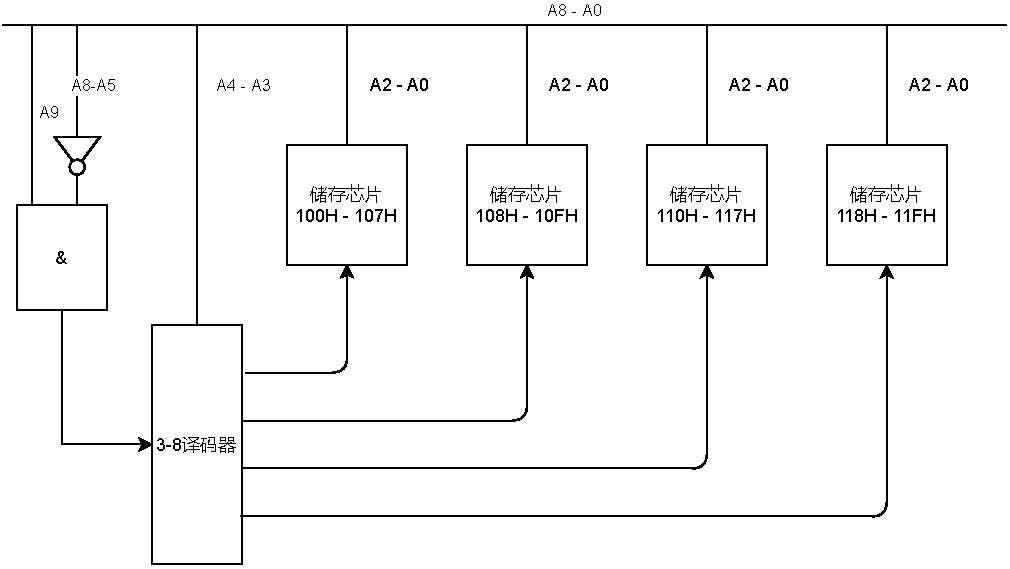
\includegraphics[width=\textwidth]{2-image}


\end{document}
